\newpage
\section*{Zielsetzung}
Im Folgenden wird der Einfluss von Parametern, wie dem Federaußendruchmesser $D_a$
und der Federwindungszahl $n$ auf die Federkonstante $R$ einer Zugfeder untersucht
und mit der Theorie sowie der verwendeten Federberechnung der Firma Schnöring verglichen.\\

Des Weiteren betrachte man den benötigten Materialeinsatz in Abhängigkeit des Federaußendurchmessers $D_a$ und 
der Windungszahl $n$.\\
Schlussendlich wird eine Aussage getroffen, wie durch die Verwendung dieser Parametern 
ein möglichst geringen Materialeinsatz für diese Zugfeder erzielt werden kann.  

 

\section{Zugfedern allgemein}
Überall wo die Krafteinwirkung nicht auf Druck, sondern auf Zug erbracht werden muss
werden Zugfedern verwendet. Trotz der benötigten Größe des Einbauraumes und der sensiblen
Stelle an den Ösen, werden Zugfedern vor allem aufgrund ihrer Knickfreiheit verwendet.
Führungselemente wie Hülsen oder Dorn sind somit überflüssig und es besteht die Möglichkeit
einer reibungsfreien zentrischen Kraftübertragung.\\
Im Folgenden soll kurz auf die verschiedenen Komponenten und Unterschiede zwischen
Zugfedern eingegangen werden:
\begin{enumerate}
    \item Federbauform und Ösenform
    \item Vorspannung
    \item Belastungsart
\end{enumerate}



\subsection{Federbauform}
Die gängigen Federbauformen für Zugfedern sind zylindrischer Form mit einer linearen
Federkennline, aber auch kegel- oder tonnenförmige Formen sind verbreitet, was vorallem
den Vorteil einer höhren Lebensdauer hat.
\begin{figure}[H]
    \centering
    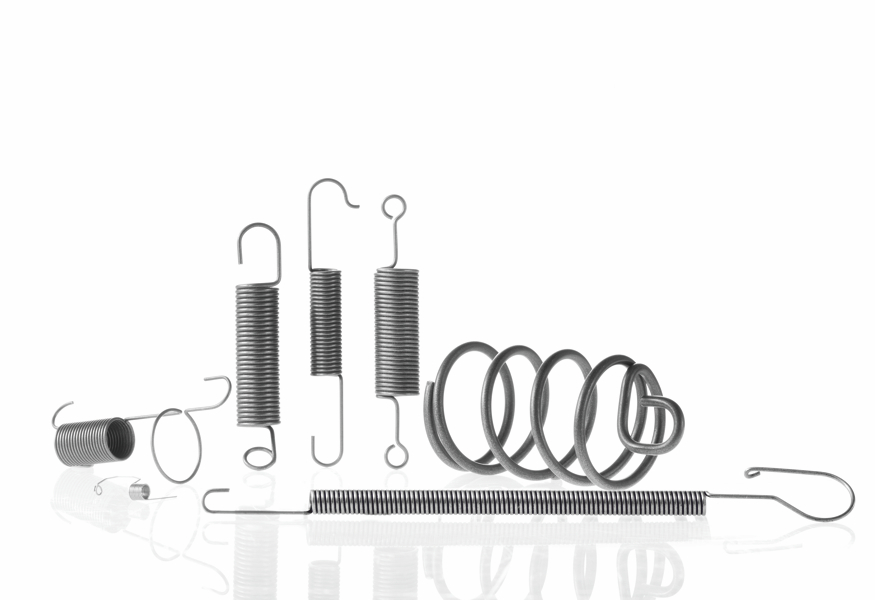
\includegraphics[width=0.6\textwidth]{bilder/Input/zugfedern_spezial.jpg}
    \caption{Spezielle Zugfedern \cite{KompZ}}
\end{figure}



\subsection{Ösenform}
Die (klassischen) Ösen der Zugfedern (bzw. die Ösenanbindung am Übergangsbogen) bilden eine schwierige Region, da es dort oftmal zu Ösenbrüchen
kommen kann. Aufgrund dessen sind Zugfedern nicht für Dauerfest-Einsätze geeignet.
Als klassisch gilt die 1/1 deutsche Öse oder der Hakenöse.
Für eine erhöhte Lebensdauer verwendet man auch einen eingerollten Gewindebolzen 
oder einen eingeschraubte Gewindestopfen.\\
Die Öse bildet dabei den zentralen Angriffspunkt für drei Kräfte: Zugbelastung, Torsionsbelastung und Biegebelastung.
\begin{figure}[H]
    \centering
    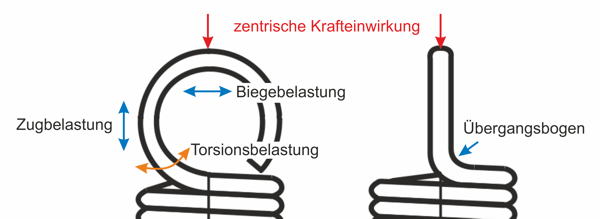
\includegraphics[width=0.6\textwidth]{bilder/Input/Oesenbelastung.jpg}
    \caption{Verschiedene Ösenbelastungen \cite{KompZ}}
\end{figure}
\begin{figure}[H]
    \centering
    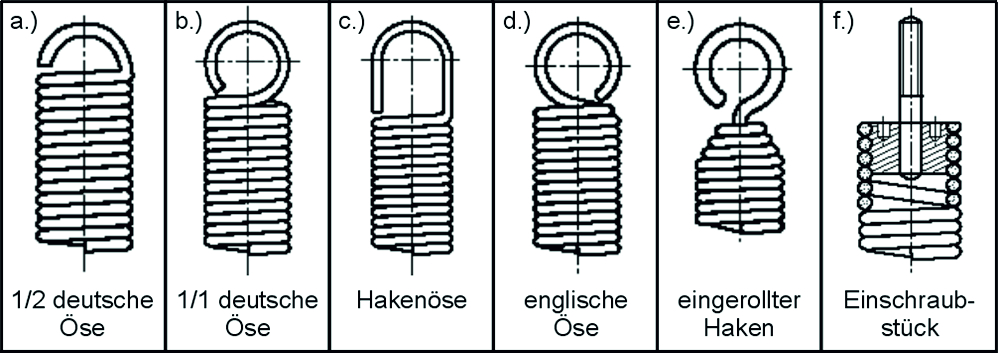
\includegraphics[width=0.6\textwidth]{bilder/Input/Oesenformen.jpg}
    \caption{Verschiedene Ösenformen \cite{AusM2}}
\end{figure}

\subsection{Beanspruchungsart}
Generell unterscheidet man zwischen einer statischen und einer dynamischen Beanspruchung.
Von einer statischen Beanspruchung einer Zugfeder spicht man bei einer zeitlich
konstanten Belastung, bzw. einer Belastung mit weniger als 10000 Hüben oder 
kleinen Hubspannungen.
Hat die Feder mehr als 10000 Lastwechsel oder Hubspannungen die konstanten und veränderlichen sind,
so spricht man von einer dynamischen Beanspruchung.

\subsection{Vorspannung}
Bei der Herstellung entsteht eine Vorspannung aufgrund eines Drilles gegen die nächste
Windung. Dadurch wird die Betriebslänge der Zugfeder minimiert, sie ist allerdings mit höhren Produktionskosten
verbunden.\\
Am Beginn des Kraft-Weg-Diagramm äußert sich die Vorspannung durch einen senkrechten Anstieg
bis $F_0$ und verläuft danach in der Neigung der Federkonstanten.  
\begin{figure}[H]
    \centering
    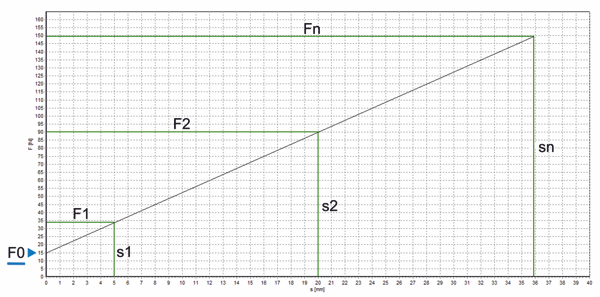
\includegraphics[width=0.6\textwidth]{bilder/Input/Vorspannung.jpg}
    \caption{Zugfeder Weg-Kraft-Diagramm \cite{KompZ}}
\end{figure}
\newpage
\section{Federberechnung Praxis}

    In der Praxis bildet für die verwendete Zugfeder (hier eine Trompetenfeder, genaueres in Abschnitt \ref{sec:feder})
    die geforderte resultierende Kraft $F1$ und $F2$ an zwei festgelegten belasteten Federlängen $L1$ und $L2$
    die Grundlage zur Federberechnung.\\

    Für die Federlänge $L0$ (also Länge der unbelasteten Feder) gibt es keinen fest vorgeschrieben Wert.\\
    Dies resultiert daraus, dass bei der Anwendung, anderes als bei Druckfedern, eine weiter zusätzliche Streckung
    der Feder gefordert ist und somit der Einbauraum größer wird.\newline

    Dabei wird in der Fertigung, um im Toleranzbereich der geforderten Federkräfte zu bleiben, $F2$ durch
    die Änderung von Federaußendruchmesser $D_a$ oder Drahtdicke $d$ korrigiert und $F1$  durch die Änderung
    von der Federlänge $L0$ und Windungszahl $n$ korriegiert.\\

    Die wichtigsten Paramter bilden dabei:
    \begin{align*}
        L1 &:& &\text{Länge 1 der belasteten Feder}\\
        F1 &:& &\text{Federkraft bei L1}\\
        L2 &:& &\text{Länge 2 der belasteten Feder}\\
        F2 &:& &\text{Federkraft bei L2}\\
        R &:& &\text{Federkonstante/-rate}\\
        d &:& &\text{Drahtdicke}\\
        D_a &:& &\text{Federaußendurchmesser}\\
        n &:& &\text{(gesamt) Wicklungszahl}\\
        n_{wirk}&:& &\text{wirkende (federnde) Wicklungszahl}\\
        s &:& &\text{Federweg}=\Delta L \\
    \end{align*}
\label{sec:praxis}























%THEORIE ----------------------------------------------------------------------
\newpage
\section{Theorie}
\begin{figure}[H]
    \centering
    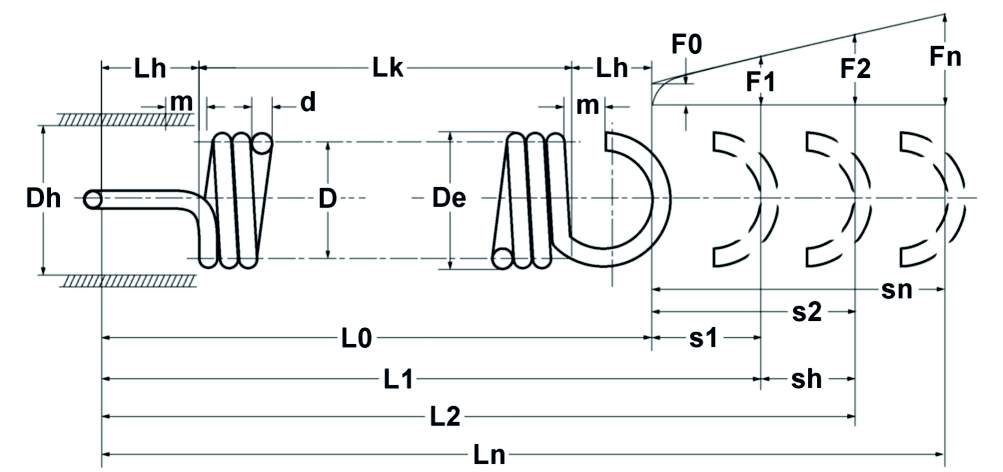
\includegraphics[width=0.6\textwidth]{bilder/Input/Zugfeder_technisch.jpg}
    \caption{Theoretisches Zugfederdiagramm \cite{AusM2}}
\end{figure}
Für zylinderische Zugfedern aus Draht mit einem Kreisquerschnitt gilt:\\\\

Die Federkonstante (auch Federrate) $R$:

\begin{equation}
    %Federrate
    R=\frac{\Delta F}{s}=\frac{Gd^4}{8D^3n_{wirk}}=\frac{F-F_0}{L},
    \label{eqn:federrate}
\end{equation}

mit der wirkende Federdicke $D$:
\begin{equation}
    D=D_a-d,
\end{equation}

Die Federkraft $F$:
\begin{equation}
    %Federkraft
    F=\frac{Gd^4s}{8D^3n_{wirk}}+F0=R \cdot s +F0,
    \label{eqn:federkraft}
\end{equation}

Die wirkende (federnde) Wicklungszahl $n_{wirk}$ für verwendete Trompetenfeder
\begin{equation}
    n_{wirk}=\frac{L0-LH}{d}    
\end{equation}

Das Wickelverhältnis $w$:
\begin{equation}
    w=\frac{D}{d},
\end{equation}

Die Federungsarbeit $W$:
\begin{equation}
    %Arbeit
    W=F0 \cdot s = \frac{1}{2}\;(F-F0) \cdot L,
    \label{eqn:federungsarbeit}
\end{equation}
\newline




% NÖTIG????? ------------------------------------
Für den Festigkeitsnachweis der Zugfeder ist die Ermittlung der Schubspannung $\tau$
nötig, welche für die dynamischen Beanspruchungen mit einem Faktor $k$ korrigiert werden müssen.

\begin{equation}
    %Schubspannung
    \tau = \frac{8DF}{\pi d^3}.
    \label{eqn:schubspannung}
\end{equation}
\begin{align}
    \tau_k &= k \cdot \tau\\
    \text{mit }k&=\frac{\frac{D}{d}+0.5}{\frac{D}{d}-0.75}
\end{align}
Für die zulässige Spannung ergib sich
\begin{equation}
    \tau_{zul}=0.45 \cdot R_m
\end{equation}
Dabei spiegelt $R_m$ die Zugfestigkeit des Federstahls wieder.\\
Ist dabei $s_n$ der zu $\tau_{zul}$ Federweg, so sollte in der Praxis nur 80\% dieses
Federweges ausgnutzt werden um Relaxation (Kraftverlust) zu vermeiden.
Also $s_{prax}=0.8 \cdot s_n$.  
%--------------------------------------------


\subsection{Theorie zur Massenberechnung}
Um die Abhängigkeit der Masse von der Windungszahl und dem Federdurchmesser zu bestimmen wird mit dem Zusammenhang zwischen Volumen und Masse gearbeitet.
\begin{equation}
    M = V \cdot \rho
\end{equation}
Um das Volumen einer Feder zu bestimmen wird die Feder als Spirale angenähert und die Trompetenenden vernachlässigt.
Für die Rechnung wird außerdem der Parameter $a$ eingeführt ,der die Länge einer Windung angibt.
\begin{equation}
    a = \frac{L}{n\cdot 2\pi}
\end{equation}
Mit der Drahtlänge $L$ und der Windungszahl n.
Der Ortsvektor für eine Spirale und seine Ableitung sind
\begin{align}
    x(t) = () && x'(t) = ()
\end{align}
Nun wird die Länge des Drahtes in Abhängigkeit von Windungszahl und Federradius bestimmt
\begin{equation}
    L = \int_{0}^{2\pi n} \sqrt{x^2+y^2+z^2}dt = t \sqrt{R^2+a^2} \; |_{0}^{2\pi n} = 2\pi n \sqrt{R^2+a^2}
\end{equation}
Nun kann die Drahtlänge in die Formel für die Masse eingesetzt werden
\begin{equation}
    M = V\cdot \rho = \pi r^2 L \rho = 2 \pi^2 r^2 n \sqrt{R^2 + a^2} \rho
\end{equation}
Also ergibt sich die Abhängigkeit für die Masse mit:
\begin{equation}
    M = A \sqrt{R^2 + \frac{B^2}{n^2}}n
\end{equation}
\label{sec:theorie}